\chapter{Основные сведения об электромагнитных переходных процессах}
\section{Основные определения}
Из всего многообразия электромагнитных переходных процессов в электрической системе наиболее распространенными являются процессы, вызванные:
\begin{enumerate} 
	\item
	включением и отключением двигателей и других приемников электроэнергии;
	\item
	коротким замыканием в системе, а также повторным включением и отключением (одновременным или 
каскадным) короткозамкнутой цепи;
	\item
	возникновением местной несимметрии в системе (например, отключение одной фазы линии передачи);
	\item
	несинхронным включением синхронных машин. 
\end{enumerate}

\so{Коротким замыканием} называют всякое не предусмотренное нормальными условиями работы замыкание между фазами, а в системах с заземленными нейтралями (или четырехпроводных)~---  также замыкание одной или нескольких фаз на землю (или на нулевой провод).

В системах с незаземленными нейтралями или с нейтралями, заземленными через специальные компенсирующие устройства, замыкание одной из фаз на землю называют \so{простым замыканием}. При этом виде повреждения прохождение тока обусловлено главным образом емкостью фаз относительно земли.

При возникновении короткого замыкания в электрической системе сопротивление цепи уменьшается (степень уменьшения зависит от положения точки короткого замыкания в системе), что приводит к увеличению токов в отдельных ветвях системы по сравнению с токами нормального режима. в свою очередь это вызывает снижение напряжений в системе, которое особенно велико вблизи места короткого замыкания.

Обычно в месте замыкания образуется некоторое переходное сопротивление, состоящее из сопротивления возникшей электрической дуги и сопротивлений прочих элементов пути тока от одной фазы к другой или от фазы на землю. Электрическая дуга возникает или с самого начала происшедшего повреждения как, например, при перекрытии или пробое изоляции, или через некоторое время, когда перегорит элемент, вызвавший замыкание. При замыканиях между фазами переходное сопротивление определяется главным образом сопротивлением электрической дуги.

\begin{wrapfigure}[17]{r}{0.4\linewidth}
\centering
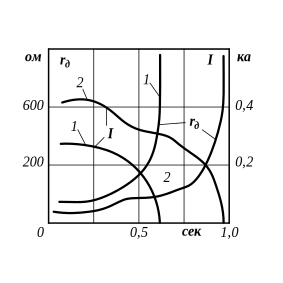
\includegraphics[width=0.95\linewidth]{pic/1-1}
\caption{Кривые изменения во времени тока и сопротивления самопогасающей открытой дуги на линии 110~\textit{кв} с деревянными опорами. \textit{1, 2} -- номера опытов.}
\label{fig:r-and-I}
\end{wrapfigure}


Когда токи достаточно велики (сотни ампер и более), сопротивление дуги приблизительно постоянно и по своему характеру почти чисто активное. С уменьшением, тока и увеличением длины дуги, что имеет место в течение переходного процесса, ее сопротивление возрастает. Наглядной иллюстрацией такого изменения могут служить графики (рис.~\ref{fig:r-and-I}), полученные экспериментально при возникновении самопогасающих дуг на линиях 110~\textit{кв} с деревянными опорами.

В ряде случаев переходные сопротивления могут быть столь малы, что практически ими можно пренебречь. Такие замыкания называют \mbox{\so{металлическими}}.

Естественно, при прочих равных условиях ток при металлическом замыкании больше, чем при наличии переходного сопротивления. Поэтому, когда требуется найти возможные наибольшие величины токов, исходят из наиболее тяжелых условий, считая, что в месте замыкания отсутствуют какие-либо переходные сопротивления\footnote{Учет переходных сопротивлений и контактных соединений при выполнении расчетов коротких замыканий для установок напряжением до 1000~\textit{в} имеет особое значение (\colorbox{red}{§ 17-5}).}.

В трехфазных системах с заземленной нейтралью различают следующие основные виды коротких замыканий в одной точке:

\begin{enumerate} 
	\item
	трехфазное;
	\item
	двухфазное;
	\item
	однофазное;
	\item
	двухфазное на землю, т.~е, замыкание между двумя фазами с одновременным замыканием той же точки на землю. 
\end{enumerate}

Трехфазное короткое замыкание является симметричным, так как при нем все фазы остаются в одинаковых условиях\footnote{При наличии переходных сопротивлений симметрия сохраняется лишь при равенстве этих сопротивлений.} Напротив, все остальные виды коротких замыканий являются несимметричными, поскольку при каждом из них фазы находятся уже в неодинаковых условиях; поэтому системы токов и напряжений при этих видах короткого замыкания в той или иной мере искажены.
	
Многолетняя аварийная статистика по союзным и зарубежным системам показывает, что при глухозаземленной нейтрали относительная вероятность различных основных видов короткого замыкания характеризуется примерными данными табл. \colorbox{red}{1-1} В той же таблице показаны рекомендуемые сокращенные обозначения каждого вида короткого замыкания.

Как видно из этой таблицы, подавляющее число коротких замыканий связано с замыканием на землю, в то время как трехфазное короткое замыкание является очень редким. Однако отсюда было бы неправильным делать вывод, что трехфазное короткое замыкание можно вообще оставить без внимания. Поскольку оно все же возможно, с ним следует считаться, тем более что оно иногда может быть решающим для окончательного суждения относительно возможности работы в условиях короткого замыкания. Само изучение процесса трехфазного короткого замыкания особенно важно в связи с тем, что применение метода симметричных составляющих позволяет величины токов и напряжений прямой последовательности любого несимметричного замыкания определять как соответственные величины при некоторых условных трехфазных замыканиях.